% arara: pdflatex: { shell: true, draft: true }
% arara: makeglossaries
% arara: biber
% arara: pdflatex: { shell: true, synctex: true }
% arara: pdflatex: { shell: true, synctex: true }

\documentclass[12pt,DIV14,BCOR10mm,a4paper,parskip=half-,headsepline,headinclude,english,ngerman,bibliography=totocnumbered]{scrreprt}

\usepackage{hshhelper_base}

\usepackage{dirtree}

%%%%%%%%%%%%%%%%%%%%%%%%%%%%%%%%%%%%%%%%%%%%%%%%%%%%%%%%%%%%%%%%%%%%%%%%%%
\begin{document}    % hier gehts los
  \thispagestyle{empty} % Titelseite

\includegraphics[width=0.2\textwidth]{Wortmarke_WI_schwarz}

   {  ~ \sffamily
  \vfill
  {\Huge\bfseries Installations- und Bedienungsanleitung}
  \bigskip

  {\Large
  Dennis Grabowski, Julius Zint, Philip Matesanz, Torben Voltmer \\[2ex]
  Masterprojekt \enquote{Entwicklung und Analyse einer sicheren \\Web-Anwendung} \\
  Wintersemester 18/19
 \\[5ex]
   \today }
}
 \vfill

  ~ \hfill
  
\includegraphics[height=0.3\paperheight]{H_WI_Pantone1665}

\vspace*{-3cm}

\tableofcontents  % Inhaltsverzeichnis

\chapter{Installation des HsH-Helpers}

\section{Mindestanforderungen}

Um den HsH-Helper ausführen zu können, müssen Sie Java 8 installiert haben.
Unterstützung für vorherige sowie spätere Java-Versionen ist nicht gegeben.

\section{Installation}

Zu dieser Installations- und Bedienungsanleitung haben Sie eine ZIP-Datei erhalten.
Diese ZIP-Datei können Sie in einem beliebigen Verzeichnis extrahieren.
Dabei entsteht folgende Ordnerstruktur: \\

\dirtree{%
.1 bin.
.2 hshhelper.
.2 hshhelper.bat.
.1 conf.
.2 application.conf.
.2 secrets.conf.
.2 logback.xml.
.2 ip\_whitelist.txt.
.2 password\_blacklist.txt.
.1 lib.
.2 hshhelper.hshhelper-1.0-SNAPSHOT.jar.
.2 // Alle Bibliotheken, von denen unsere Applikation abhängt.
}

\bigskip
Im \texttt{bin}-Ordner befinden sich Startskripte für Windows sowie UNIX.
Diese können auf der Kommandozeile ausgeführt werden, um die HsH-Helper Applikation zu starten.

\chapter{Betrieb}

Bevor Sie den HsH-Helper starten können, sollten Sie verifizieren, dass der Applikation ein sicheres Geheimnis vorliegt.
Dieses ist in der \texttt{conf/secrets.conf} unter dem Schlüssel \texttt{play.http.secret.key} persistiert.
Um ein möglichst sicheres Geheimnis zu generieren, könnten sie die Bibliothek OpenSSL verwenden.

\begin{lstlisting}[label=server-private-key, caption={OpenSSL-Befehl zum Erstellen eines privaten Schlüssels}, captionpos=b]
\\ RSA
openssl genpkey -algorithm RSA -pkeyopt rsa_keygen_bits:4096 -pkeyopt rsa_keygen_pubexp:65537 > rsa-4096-private-key.pem
\\ EdDSA - erst ab OpenSSL v1.1.1
openssl genpkey -algorithm Ed25519 -out ed25519-private-key.pem
\\ ECC
openssl genpkey -algorithm EC -pkeyopt ec_paramgen_curve:P-384 -pkeyopt ec_param_enc:named_curve > p384-private-key.pem
\end{lstlisting}

Das generierte Geheimnis müssen sie dann aus der jeweiligen Datei kopieren und in der \texttt{conf/secrets.conf}-Datei speichern unter dem Schlüssel \texttt{play.http.secret.key}.
Wichtig ist, dass Sie auf gar keinen Fall das Secret "changeme" nennen, da sonst der HsH-Helper nicht starten wird.
Danach ist der HsH-Helper startbereit.

Um dem HsH-Helper zu starten, müssen Sie sich auf der Kommandozeile ihres Betriebssystems in den Ordner bewegen, in dem Sie zuvor den HsH-Helper extrahiert haben.
Mit folgenden Befehlen können Sie dann von dort aus den HsH-Helper starten:

\begin{lstlisting}[label=server-operation, caption={Kommandozeilenbefehle zum Ausführen der Applikation}, captionpos=b]
// UNIX
$ ./bin/hshhelper
// Windows
> bin\hshhelper.bat
\end{lstlisting}

Nach dem Start der Applikation werden Sie auf der Kommandozeile von einigen Logging-Ausgaben begrüßt.
Der Server ist betriebsbereit, sobald Sie folgende Zeile in ihrem Kommandozeileninterface sehen: \\
\texttt{[info] p.c.s.AkkaHttpServer - Listening for HTTP on /0:0:0:0:0:0:0:0:9000}

Danach können Sie den HsH-Helper von ihrem Browser erreichen, in dem Sie \texttt{\url{http://localhost:9000}} ansurfen, sofern Sie die IP-Adresse / Hostname sowie Port nicht verändert haben (siehe \autoref{manual:configuration})

Während des Hochfahrens der Applikation wird ein Ordner namens \texttt{logs/} in dem Applikationsverzeichnis erstellt.
Innerhalb dieses Verzeichnisses befinden sich die Zugriffs- und Applikationslogs.

\chapter{Konfiguration}
\label{manual:configuration}

Der HsH-Helper ist an verschiedenen Punkten konfigurierbar.
Die Werkseinstellungen können Sie notfalls auch dem Anhang \ref{app-default-configuration} entnehmen, sofern Sie anders nicht mehr darauf zugreifen können.
Die hier genannten Einstellungen sind Einstellungen, die wir unterstützen und dessen Sicherheit wir garantieren können.
Sollten Sie aus irgendwelchen Gründen bestimmte Zusatzfeatures\footnote{Menge aller möglichen Einstellungen, siehe \url{https://www.playframework.com/documentation/2.6.x/ProductionConfiguration}} nutzen wollen, sind Sie auf sich allein gestellt.

Für den Fall, dass Sie die Applikation mit einer komplett separaten Konfigurationsdatei ausführen wollen, so können Sie diese beim Start der Applikation auf der Kommandozeile hinzufügen, in dem Sie folgenden Parameter anhängen: \\
\texttt{-Dconfig.file=/path/to/config/file.conf}

\section{Serverkonfiguration}

\subsection{Dateien größer als ~200 MB hochladen}

Falls Sie während des Betriebs des HsH-Helpers den Nutzern erlauben möchten, Dateien hochzuladen, dessen Größe mehr als 200 Megabyte beträgt, so müssen Sie innerhalb der Konfigurationsdatei 2 Einstellungen ändern.
Bei diesen Einstellungen handelt es sich um die maximale Größe eines HTTP-Pakets, die das Play Framework verarbeiten darf.
Rechnen Sie also sicherheitshalber ein paar Megabyte mehr dazu.

\begin{lstlisting}[label=server-max-file-upload, caption={"Dateigröße und HTTP-Paketgröße"-Einstellung innerhalb der Konfigurationsdatei}, captionpos=b]
play.http.parser.maxDiskBuffer = 200MB
parsers.anyContent.maxLength = 200MB
\end{lstlisting}

\subsection{IP-Adresse auf eine Whitelist setzen, so dass sie nicht blockiert wird}

Sollten Sie wünschen, bestimmte IP-Adressen auf eine Whitelist zu setzen, damit diese nicht von unserer \enquote{Login-Firewall} blockiert wird, so müssen sie diese IP-Adressen in die \texttt{conf/ip\_whitelist.txt} schreiben.
Dabei sollte jede IP-Adresse auf eine eigene Zeile geschrieben werden.
Diese Funktionalität eignet sich besonders, um eine Universität freizuschalten, damit die Studenten, die gegebenfalls mit der selben IP-Adresse ihre Seite ansurfen nicht vom HsH-Helper ausgeschlossen werden können.

\subsection{Server auf einer anderen IP-Adresse/einem anderen Port laufen lassen}

Sollten Sie die IP-Adresse oder den Port ändern wollen, auf dem der HsH-Helper standardmäßig läuft, so müssen Sie das beim Start der Applikation angeben, in dem Sie folgende Parameter auf der Kommandozeile hinzufügen: \\
\texttt{-Dhttp.port=1234 -Dhttp.address=123.123.123.123}

Bei einer Anpassung der Adresse müssen Sie zusätzlich die Content Security Policy anpassen.
Wie das geht, können Sie in \autoref{server-adjust-csp} nachlesen.

\subsection{Server auf einer anderen Domäne als \texttt{localhost} anbieten}

Sollten Sie den HsH-Helper auf einer externen Domäne anbieten wollen, so müssen Sie in der Konfigurationsdatei folgende Einstellungen ändern, damit die Applikation auch funktional korrekt weiterläuft.

Zunächst müssen Sie die Content Security Policy (CSP) anpassen.\label{server-adjust-csp}
Beim Single Sign-On wird eine JavaScript-Funktion verwendet, um nur die Anmeldeinformationen des Netzdienst zu laden, zu welchem sich ein Nutzer gerade versucht zu verbinden.
Dadurch garantieren wir, dass nicht alle hinterlegeten Anmeldeinformationen aler Netzdienste eines Nutzers geladen werden müssen.
In unserer CSP erlauben wir kein JavaScript ausser von einem bestimmten Pfad des Servers, siehe \autoref{server-foreign-domain}.
Dazu müssen die Hostnamen / IP-Adressen in der Policy-Deklaration (\texttt{http://localhost:9000/assets/js/ http://127.0.0.1:9000/assets/js/}) mit den passenden Domänennamen / IP-Adressen ersetzt werden.

Zusätzlich müssen Sie erlauben, dass Clients von ausserhalb ihren Server ansurfen können, siehe \autoref{server-subsubsection-different-host}.

\begin{lstlisting}[label=server-foreign-domain, caption={"Content Security Header"-Einstellung innerhalb der Konfigurationsdatei}, captionpos=b]
play.filters {
  headers {
    contentSecurityPolicy = "default-src 'self'; script-src https://www.google.com/recaptcha/ https://www.gstatic.com/recaptcha/ http://localhost:9000/assets/js/ http://127.0.0.1:9000/assets/js/; frame-src https://www.google.com/recaptcha/; img-src 'self' data:"
  }
}
\end{lstlisting}

\subsection{Server von einem anderen Host als \texttt{localhost} ansteuern}
\label{server-subsubsection-different-host}

Damit Clienten, die sich nicht auf ihrem lokalen Host befinden, den HsH-Helper ansteuern können, müssen Sie entweder deren Hostnamen / IP-Adressen in der Einstellung, siehe \autoref{server-foreign-allowed-hosts}, explizit eintragen oder die Einstellung \texttt{allowed} vollständig auskommentieren, damit jeder Host Zugriff hat.

\begin{lstlisting}[label=server-foreign-allowed-hosts, caption={"Erlaubte Hosts"-Einstellung innerhalb der Konfigurationsdatei},captionpos=b]
play.filters {
  hosts {
    allowed = ["localhost:9000", "localhost:19001", "127.0.0.1:9000"]
  }
}
\end{lstlisting}

\subsection{Testing: reCAPTCHA automatisierbar testen}

Für den Fall, dass Sie den HsH-Helper automatisierbaren Tests unterziehen wollen, ihnen dabei aber das reCAPTCHA in die Quere kommt, besteht die Möglichkeit, ein reCAPTCHA extra für Testzwecke einzubauen.
Dazu müssen Sie den geheimen Schlüssel sowie den Schlüssel der Seite in der \texttt{secrets.conf} auszutauschen.
Hierfür entnehmen Sie bitte der Seite \url{https://developers.google.com/recaptcha/docs/faq\#id-like-to-run-automated-tests-with-recaptcha-what-should-i-do} die Schlüssel, die Google anbietet, um automatisierbare Tests durchzuführen.
\textbf{Vorsicht:} Bevor Sie das tun, sollten sie die alten Schlüssel sicher abspeichern.
Ohne diese können Sie kein echtes reCAPTCHA verwenden.

\section{Datenbankkonfiguration}

Unsere Applikation bietet nur Unterstützung für die Datenbank \texttt{h2}.
Bei anderen Datenbanken kann nicht garantiert werden, dass die Applikation überhaupt startet.
Ebenso ist die Sicherheit der Applikation unter Verwendung einer anderen Datenbank nicht gewährleistet.

\subsection{Verbindungsmodus}

Mit Werkseinstellungen wird die Datenbank im Hauptspeicher persistiert (In-Memory Database).
Dies erhöht die Sicherheit, da die Datenbank an den Speicher des Prozesses gebunden ist, und somit kein anderer Prozess darauf zugreifen kann.
Nachteil ist allerdings, dass dadurch bei einem Applikationsneustart oder Rechnerabsturz der gesamte Datenbankinhalt verloren geht.

Offiziell unterstützen wir nur die In-Memory Database.
Sollten Sie dennnoch den Wunsch haben, die Datenbank über die Grenzen einer Applikationslaufzeit zu persistieren, so müssen Sie die Konfigurationsdatei anpassen, siehe \ref{db-connection-mode}.

\begin{lstlisting}[label=db-connection-mode, caption={Einstellung innerhalb der Konfigurationsdatei zum Anpassen des Verbindungsmodus der verwendeten Datenbank},captionpos=b]
db {
  default.url = "jdbc:h2:mem:hshhelper;mode=mysql"
}
\end{lstlisting}

\begin{sloppypar}
Um die Datenbank in einer Datei zu persistieren, die für einen späteren Applikationsstart wieder verwendet werden kann, sollten Sie \texttt{default.url} auf \texttt{"jdbc:h2:file:./hsh-helper;mode=mysql"} (inkl. Anführungsstriche) setzen.
\end{sloppypar}
Andere, mögliche Verbindungsmodi können der \texttt{h2}-Dokumentation\footnote{Für weitere Verbindungsmodi siehe \url{http://www.h2database.com/html/features.html\#database\_url}} entnommen werden.

\chapter{Bedienungsanleitung}

\section{Einstellungen}

In Anhang \autoref{manual:user-settings} sieht man die Benutzersicht für die Zusatzfunktionalitäten \enquote{Session-Timeout anpassen}, \enquote{Passwort ändern}, \enquote{Zwei-Faktor Authentisierung}.
Diese sind zusammengefasst unter \enquote{Einstellungen} zu finden.

\subsection{\enquote{Session Timeout} anpassen}

Bei Werkseinstellungen ist der Session Timeout auf das absolute Minimum, 5 Minuten, gesetzt.
Für Nutzer, welche diesen Timeout als zu kurz empfinden, ist es möglich, ihn auf eine andere Zahl zu setzen, bis auf ein Maximum von einem Tag.
Um dies zu bewerkstelligen, muss der Nutzer nur angeben, wie viele Minuten lang eine Session gültig sein sollte.

\subsection{Passwort ändern}

Sofern ein Nutzer wünscht, sein eigenes Passwort zu ändern, so kann er dies tun in dem er sein aktuelles sowie das neue Passwort eingibt.
Wegen der Implementation der verschlüsselten Netzdienstanmeldeinformationen ist es leider nötig, das aktuelle Passwort einzugeben.

\subsection{Zwei-Faktor Authentisierung aktivieren}

Falls ein Nutzer zusätzliche Sicherheit wünscht, so kann er eine Zwei-Faktor-Authentisierung aktivieren.
Beim Klick auf den Knopf zum Aktivieren, wird ein Nutzer auf eine andere Ansicht (siehe Anhang \ref{manual:two-auth-factor}) weitergeleitet, auf welcher ihm ein QR-Code angezeigt wird.
Dieser QR-Code enthält ein Geheimnis, welches von einer Handy-Applikation wie \href{https://authy.com/}{Authy}
 oder \href{https://play.google.com/store/apps/details?id=com.google.android.apps.authenticator2\&hl=en}{Google Authenticator} gescannt werden kann.
Nachdem der Nutzer diesen QR-Code mit der Applikation seiner Wahl gescannt hat, muss er sich einen neues Aktivierungstoken generieren lassen und dieses angeben, um die Zwei-Faktor-Authentisierung für sein Nutzerkonto zu aktivieren.

\section{Sessions}

In Anhang \autoref{manual:sessions} sieht man die Benutzersicht für die Zusatzfunktionalität \enquote{Sessions verwalten}.
Hier ist es einem Nutzer möglich, vorherige erfolgreiche Logins zu betrachten sowie alle aktuell aktiven Sessions zu sehen und sofern gewünscht auch zu invalidieren.
Beim Invalidieren einer Session durch den Klick auf den Button neben der jeweiligen Session wird diese aus der Datenbank entfernt.
Sollte jemand diese Session gerade verwenden, so wird dieser Verwender dieser Session ausgeloggt.
Achtung: Es ist möglich, seine eigene, gerade aktive Session zu invalidieren.
Dadurch loggt man sich effektiv selbst aus.

\printbibliography

% Can be used to add a list of acronyms with their description
%\glsaddall
%\deftranslation{to=German}{Acronyms}{Abkürzungsverzeichnis}
%\deftranslation{to=German}{Glossary}{Glossar}
\printacronyms[title=Abkürzungsverzeichnis,toctitle=Abkürzungsverzeichnis]
\printglossary[title=Glossar,toctitle=Glossar,type=main]

%\addcontentsline{toc}{chapter}{\listfigurename}
% Insert list of figures, if a figure has been added to document
\iftotalfigures
  \listoffigures
\fi

%s\addcontentsline{toc}{chapter}{\listtablename}
% \listoftables       % Tabellenverzeichnis

\begin{appendices}

\chapter{Werkseinstellungen unserer Applikation: \texttt{conf/application.conf}}
\label{app-default-configuration}
\lstinputlisting{../src/conf/application.conf}


\chapter{Benutzersicht für Zusatzfunktionalität \enquote{Benutzereinstellungen}}
\begin{figure}[!htb]
	\hspace*{-1cm}
	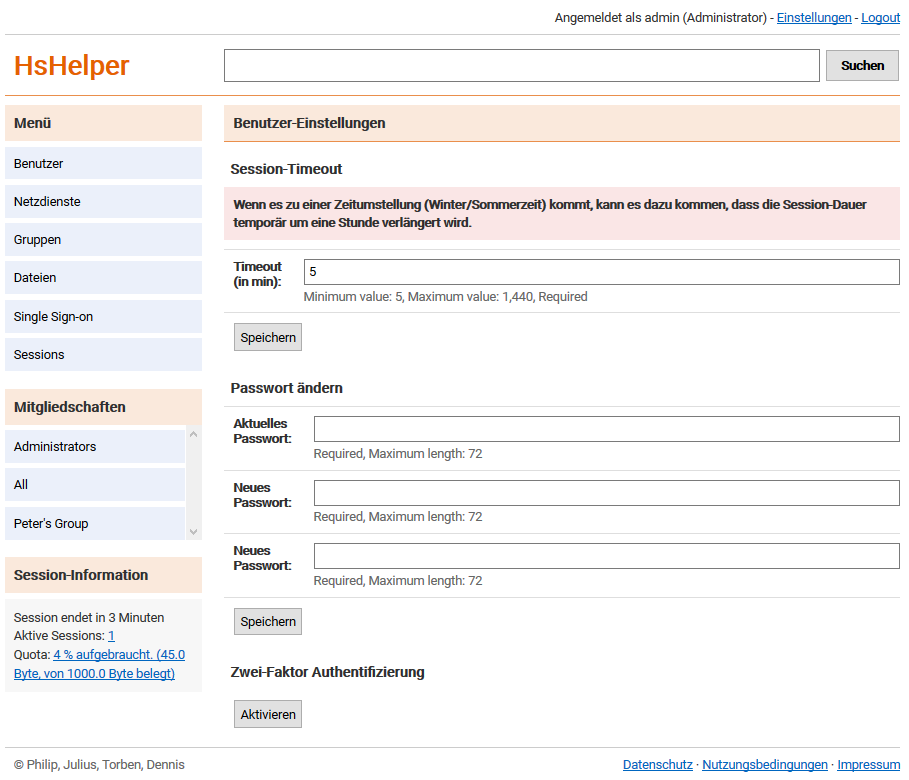
\includegraphics[width=0.8\paperwidth]{resources/settings-manual.png}
	\label{manual:user-settings}
\end{figure}

\chapter{Benutzersicht für Zusatzfunktionalität \enquote{Zwei-Faktor Authentisierung}}
\begin{figure}[!htb]
	\hspace*{-1cm}
	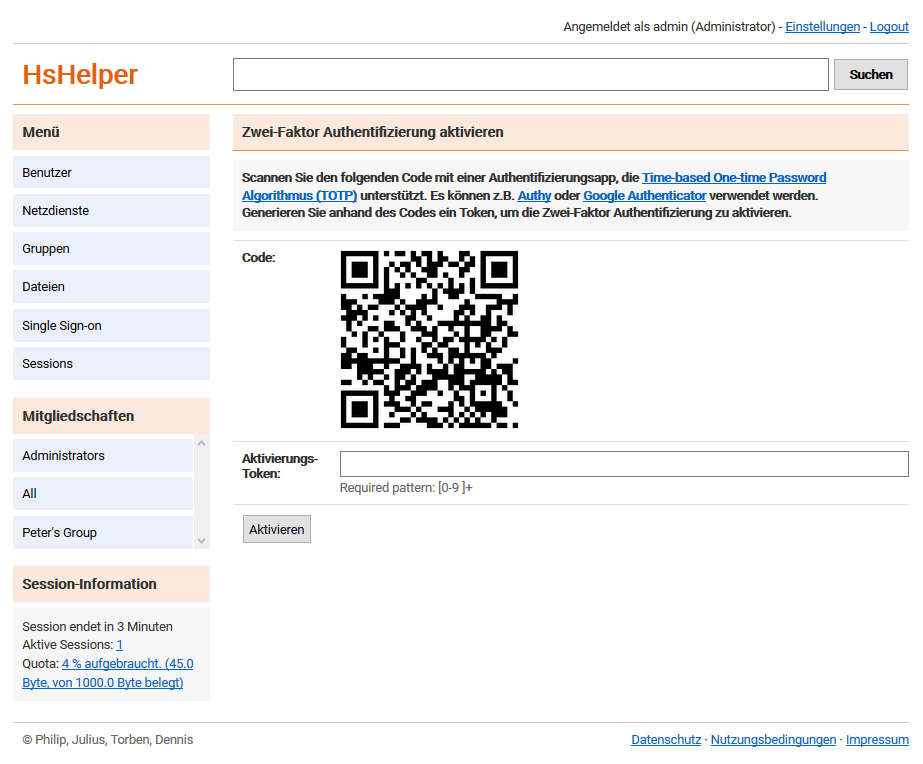
\includegraphics[width=0.8\paperwidth]{resources/two-auth-factor-manual.png}
	\label{manual:two-auth-factor}
\end{figure}

\chapter{Benutzersicht für Zusatzfunktionalität \enquote{Sessions verwalten}}
\begin{figure}[!htb]
	\hspace*{-1cm}
	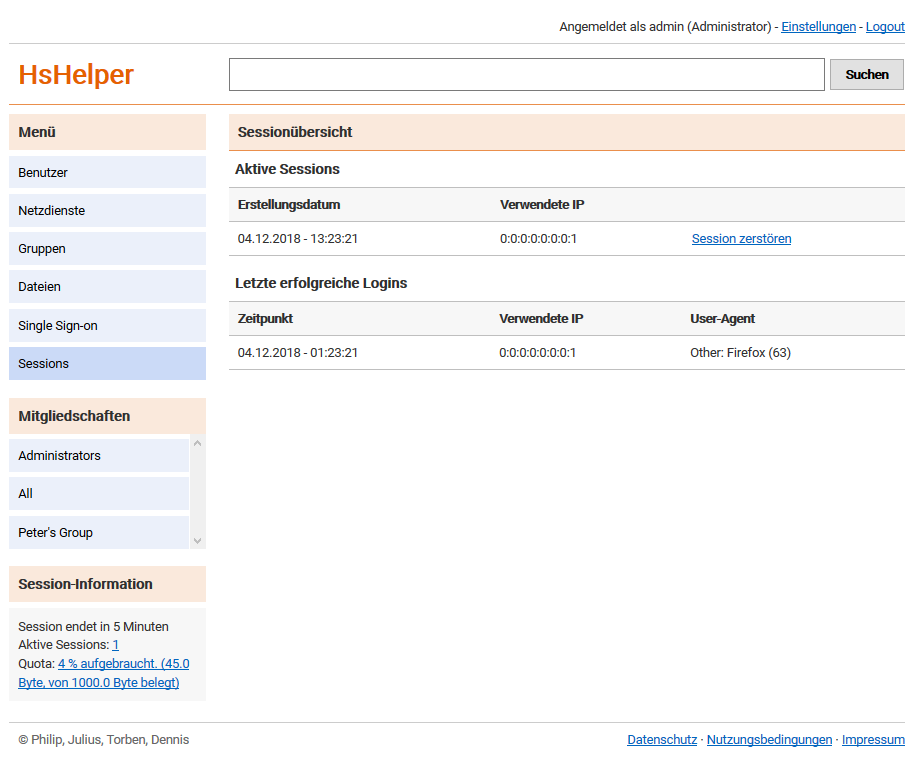
\includegraphics[width=0.8\paperwidth]{resources/sessions-manual.png}
  \label{manual:sessions}
\end{figure}


\end{appendices}

\end{document}
